\chapter{系统总体设计}\label{chap:systemoveral}

本章将介绍系统的总体设计结构,包括对 NVDLA 的详细介绍,选用的 FPGA 开发板卡资源介绍,NVDLA 与 ARM互联的解决方案。

\section{NVDLA}

NVDLA 是 NVIDIA 公司在2017年年末公布并且开源的,遗憾的是该项目自公布完成一年后便草草停止了维护。NVDLA 是一款模块化、可配置的神经网络推理加速器框架。通过核心MAC阵列、与查找表逻辑,NVDLA 可以支持深度神经网络算子,已经支持的有:

\begin{itemize}
    \item 卷积运算
    \item 激活函数
    \item 池化
    \item 归一化
\end{itemize}

实际上,由于NVDLA是完全开源的,完全可以自己手动添加相关算子的硬件逻辑。

\subsection{NVDLA 硬件结构分析}

前文中提到,NVDLA 具有模块化的属性,这很有助于我们理解加速器的工作流程,如图~\ref{fig:NVDLA Architecture}所示,NVDLA 的各个模块可以独立、同时工作。

\begin{figure}[!htbp]
    \centering
    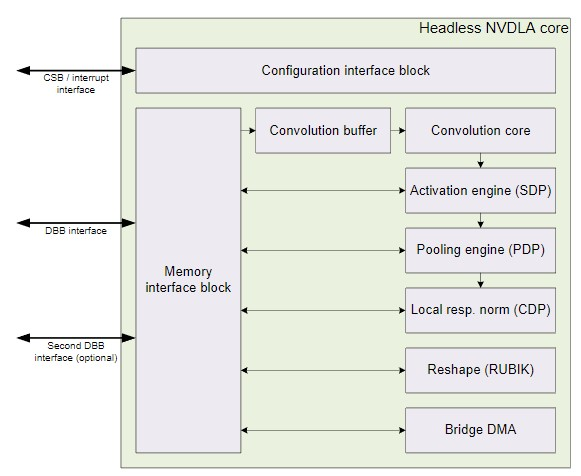
\includegraphics[width=0.7\textwidth]{NVDLA Architecture.jpg}
    \caption{NVDLA 体系结构}
    \label{fig:NVDLA Architecture}
\end{figure}

\begin{itemize}
    \item 卷积引擎配置了卷积 Buffer,在使能卷积运算的时候,需要先通过寄存器配置给出 Input Image 与 Weights 在内存上的地址,然后将数据缓存到 Buffer 中来进行运算,减少访存的开销。NVDLA 支持两种卷积模式:
    \begin{itemize}
        \item 直接卷积,及标准的卷积,可以通过 MAC 阵列并行加速。
        \item Winograd 快速卷积,从算法层面通过共用权重来减少运算量。
    \end{itemize}
    卷积引擎的核心是 MAC 阵列,该阵列的大小是可配置的,本文使用阵列大小为 8x8 。卷积的结果不可以直接写回内存,必须经过SDP,及激活函数层,其他引擎则没有这个限制。
    \item 除去卷积引擎之外,NVDLA 一共还有五个引擎,他们是负责完成激活函数的 SDP 引擎,负责完成池化操作的 PDP 引擎,负责完成 LRN 操作的CDP引擎,做图形 Reshape 的 RUBIK 引擎,最后,NVDLA 设计还提供了一个 BDMA 引擎,用来在 DRAM 和高速存储之间搬移数据。
\end{itemize}

NVDLA 在外侧暴露出四个接口,它们分别是 CSB 总线,主存储接口、高速存储接口、中断接口。

\begin{itemize}
    \item 寄存器配置总线(Configuration Space Bus Interface,CSB) ,用来读写 NVDLA 的寄存器,对于 CSB 总线,我们不甚讲解,其在读写地址的时候需要做移位来压缩指令大小,NVDLA 提供了 csb2apb 转换电路,在读写的时候使用该电路包裹即可利用 APB 总线协议读写 NVDLA 的寄存器。
    \item 主存储接口(Data Backbone interface,DBB),用来访存,该接口使用的协议为 AXI4 总线协议,可以挂载在 AXI4 接口的存储控制器上,在本文中,我们将其挂载到片上的 DDR 存储,与 ARM 处理器共享内存。
    \item 高速存储接口(high-bandwidth interface),可以外接第二块 SRAM 作为辅存储,存储中间数据,降低访存瓶颈。
    \item 中断接口(Interrupt interface),NVDLA 不仅支持通过寄存器查询的方式查询任务是否完成,也支持产生硬件中断,方便我们编写驱动程序。
\end{itemize}

\subsection{NVDLA 自定义配置}

在本设计中,我们使用官方提供的 small 配置,即最精简的NVDLA配置,该配置有如下特点:

\begin{enumerate}
    \item 最小化 MAC 阵列,本设计将 NVDLA 的 MAC 阵列大小配置为 8 * 8。
    \item 关闭高速存储接口,只使用主存储接口。
    \item 仅支持 INT8 格式的 MAC 运算。
    \item 不支持权重压缩。
    \item 不支持 WINOGRAD 快速卷积。
    \item 不支持 Reshape 特征图。
\end{enumerate}

\subsection{NVDLA 软件工具链}

如图~\ref{fig:Software Stack},NVDLA 的软件工具链分为 Compiler 和 Runtime 两个部分。

\begin{figure}[!htbp]
    \centering
    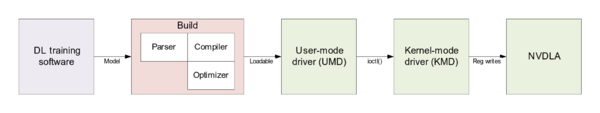
\includegraphics[width=0.9\textwidth]{Software Stack.png}
    \caption{NVDLA 软件栈}
    \label{fig:Software Stack}
\end{figure}

Compiler 与硬件无关,可以在主机运行。它可以接受其他深度神经网络训练框架训练完成的模型,完成一些硬件无关的优化,例如算子融合、数据重用等,并且使用 FlatBuffers 将处理结果封装成 Loadable 数据流文件。

Runtime 与硬件紧密结合,其负责接受 Compiler 生成的 Loadable 文件,调度加速器程序,自动分配内存,自动配置寄存器,自动处理中断。而 Runtime 内部又被划分为两个部分,UMD 和 KMD吗,分别对应了 Linux 的用户态驱动与内核驱动。

\begin{itemize}
    \item 用户态驱动程序(USER MODE DRIVER,UMD)由 C++ 编写,负责解析 Loadable 文件,分配内存,并将上下文封装成一个 Task,最后发送给底层的 KMD 程序执行。
    \item 内核态驱动程序(e KERNEL MODE DRIVER)由 C 语言编写,是 NVDLA 固件的驱动程序,他是真正与 NVDLA 进行交互的部分。
\end{itemize}

软件栈设计的详细内容,我们将在软件实现这一章详细讨论。

\section{验证平台}

NVDLA 加速器设计需要挂载到 Linux 内核上,所以本设计需要一款通用处理器作为主控,并且移植 Linux 操作系统。并且,考虑到本设计采用的 small 配置需要7万以上的查找表资源。则可供选型的器件型号有:

\begin{enumerate}
    \item ZYNQ 7000 系列,该芯片集成了一块双核32位 ARM A9 处理器作为主控制器,而 FPGA 侧的资源随芯片的型号不同而不同,想要实现 NVDLA 至少需要使用到 ZYNQ 7045 器件。
    \item ZYNQ MPSoc 系列,该芯片集成了一块多核的64位的 ARM A53 处理器作为主控制器,性能相较于 ZYNQ 7000 器件强,官方开发板卡的价格在2万左右。
    \item 纯FPGA逻辑器件,如官方板卡 VCU118,有足够大的LUT资源,可以将 RISC-V 处理器与 NVDLA 一起实现,并在 RISC-V 处理器上移植 Riscv-Linux,但缺点是板卡价值近十万元,十分昂贵,由于使用了 RISC-V 处理器,开发周期较长。
\end{enumerate}

综合以上,本设计选用的器件型号为 XC7Z045-2FFG900I,开发板卡为如图~\ref{fig:ZYNQ 7045}的第三方板卡,价格为三千多元人民币。

\begin{figure}[!htbp]
    \centering
    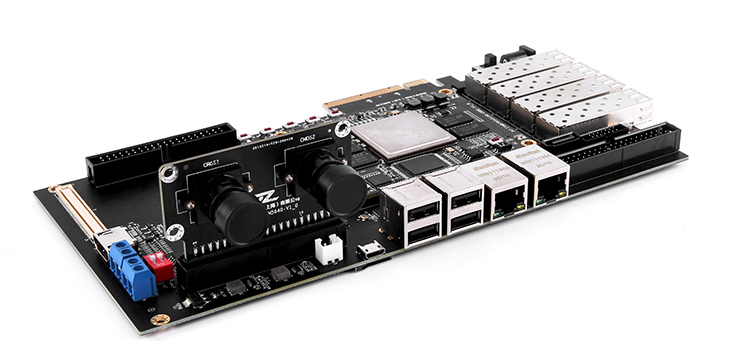
\includegraphics[width=0.9\textwidth]{ZYNQ 7045.jpeg}
    \caption{ZYNQ 7045 开发板}
    \label{fig:ZYNQ 7045}
\end{figure}

\section{AXI4 总线互联}

在 Xilinx 的设计工具中提供的 IP 核大多使用 AXI4 总线来实现各级之间的逻辑控制和数据传输。前文中提到,NVDLA 亦是使用 AXI4 总线访问存储,无疑极大方便了我们的设计,但是 NVDLA 的控制总线协议不是 AXI4 协议,在本设计中,其通过 csb2apb 电路将 CSB 协议转换为 APB 总线协议,在 Vivado 设计中,我们使用 Xilinx 官方提供给的 APB2AXI Bridge IP 将 APB 总线再转换为 AXI4 总线挂载到 ARM 处理器上。

